%%
%% This is file `sample-authordraft.tex',
%% generated with the docstrip utility.
%%
%% The original source files were:
%%
%% samples.dtx  (with options: `authordraft')
%% 
%% IMPORTANT NOTICE:
%% 
%% For the copyright see the source file.
%% 
%% Any modified versions of this file must be renamed
%% with new filenames distinct from sample-authordraft.tex.
%% 
%% For distribution of the original source see the terms
%% for copying and modification in the file samples.dtx.
%% 
%% This generated file may be distributed as long as the
%% original source files, as listed above, are part of the
%% same distribution. (The sources need not necessarily be
%% in the same archive or directory.)
%%
%% Commands for TeXCount
%TC:macro \cite [option:text,text]
%TC:macro \citep [option:text,text]
%TC:macro \citet [option:text,text]
%TC:envir table 0 1
%TC:envir table* 0 1
%TC:envir tabular [ignore] word
%TC:envir displaymath 0 word
%TC:envir math 0 word
%TC:envir comment 0 0
%%
%%
%% The first command in your LaTeX source must be the \documentclass command.
\documentclass[sigconf, nonacm]{acmart}
%% NOTE that a single column version may required for 
%% submission and peer review. This can be done by changing
%% the \doucmentclass[...]{acmart} in this template to 
%% \documentclass[manuscript,screen]{acmart}
%% 
%% To ensure 100% compatibility, please check the white list of
%% approved LaTeX packages to be used with the Master Article Template at
%% https://www.acm.org/publications/taps/whitelist-of-latex-packages 
%% before creating your document. The white list page provides 
%% information on how to submit additional LaTeX packages for 
%% review and adoption.
%% Fonts used in the template cannot be substituted; margin 
%% adjustments are not allowed.

%%
%% \BibTeX command to typeset BibTeX logo in the docs
\AtBeginDocument{%
  \providecommand\BibTeX{{%
    \normalfont B\kern-0.5em{\scshape i\kern-0.25em b}\kern-0.8em\TeX}}}

%% Rights management information.  This information is sent to you
%% when you complete the rights form.  These commands have SAMPLE
%% values in them; it is your responsibility as an author to replace
%% the commands and values with those provided to you when you
%% complete the rights form.
% \setcopyright{acmlicensed}
% \copyrightyear{2018}
% \acmYear{2018}
% \acmDOI{XXXXXXX.XXXXXXX}
\setcopyright{none}
\settopmatter{printacmref=false} % Removes citation information below abstract
\renewcommand\footnotetextcopyrightpermission[1]{} % removes footnote with conference information in first column
\pagestyle{plain}

%% These commands are for a PROCEEDINGS abstract or paper.
% \acmConference[Conference acronym 'XX]{Make sure to enter the correct
%   conference title from your rights confirmation emai}{June 03--05,
%   2018}{Woodstock, NY}
%
%  Uncomment \acmBooktitle if th title of the proceedings is different
%  from ``Proceedings of ...''!
%
%\acmBooktitle{Woodstock '18: ACM Symposium on Neural Gaze Detection,
%  June 03--05, 2018, Woodstock, NY} 
% \acmISBN{978-1-4503-XXXX-X/18/06}


%%
%% Submission ID.
%% Use this when submitting an article to a sponsored event. You'll
%% receive a unique submission ID from the organizers
%% of the event, and this ID should be used as the parameter to this command.
%%\acmSubmissionID{123-A56-BU3}

%%
%% For managing citations, it is recommended to use bibliography
%% files in BibTeX format.
%%
%% You can then either use BibTeX with the ACM-Reference-Format style,
%% or BibLaTeX with the acmnumeric or acmauthoryear sytles, that include
%% support for advanced citation of software artefact from the
%% biblatex-software package, also separately available on CTAN.
%%
%% Look at the sample-*-biblatex.tex files for templates showcasing
%% the biblatex styles.
%%

%%
%% For managing citations, it is recommended to use bibliography
%% files in BibTeX format.
%%
%% You can then either use BibTeX with the ACM-Reference-Format style,
%% or BibLaTeX with the acmnumeric or acmauthoryear sytles, that include
%% support for advanced citation of software artefact from the
%% biblatex-software package, also separately available on CTAN.
%%
%% Look at the sample-*-biblatex.tex files for templates showcasing
%% the biblatex styles.
%%

%%
%% The majority of ACM publications use numbered citations and
%% references.  The command \citestyle{authoryear} switches to the
%% "author year" style.
%%
%% If you are preparing content for an event
%% sponsored by ACM SIGGRAPH, you must use the "author year" style of
%% citations and references.
%% Uncommenting
%% the next command will enable that style.
%%\citestyle{acmauthoryear}

%%
%% end of the preamble, start of the body of the document source.
\begin{document}

%%
%% The "title" command has an optional parameter,
%% allowing the author to define a "short title" to be used in page headers.
\title{Fraud Credit Card Transaction Detection}
\subtitle{DSCI 303 Final Project}

%%
%% The "author" command and its associated commands are used to define
%% the authors and their affiliations.
%% Of note is the shared affiliation of the first two authors, and the
%% "authornote" and "authornotemark" commands
%% used to denote shared contribution to the research.
\author{(Apple) Xuanchen Li}
% \authornote{Both authors contributed equally to this research.}
\email{xl102@rice.edu}
% \orcid{1234-5678-9012}
% \author{G.K.M. Tobin}
% \authornotemark[1]
% \email{tf18@rice.edu}
\affiliation{%
  \institution{Rice University}
  % \streetaddress{P.O. Box 1212}
  % \city{Dublin}
  % \state{Ohio}
  % \country{USA}
  % \postcode{43017-6221}
}

\author{(Derek) Tiancheng Fu}
% \authornote{Both authors contributed equally to this research.}
\email{tf18@rice.edu}
% \orcid{1234-5678-9012}
% \author{G.K.M. Tobin}
% \authornotemark[1]
% \email{tf18@rice.edu}
\affiliation{%
  \institution{Rice University}
  % \streetaddress{P.O. Box 1212}
  % \city{Dublin}
  % \state{Ohio}
  % \country{USA}
  % \postcode{43017-6221}
}

% \author{Lars Th{\o}rv{\"a}ld}
% \affiliation{%
%   \institution{The Th{\o}rv{\"a}ld Group}
%   \streetaddress{1 Th{\o}rv{\"a}ld Circle}
%   \city{Hekla}
%   \country{Iceland}}
% \email{larst@affiliation.org}

% \author{Valerie B\'eranger}
% \affiliation{%
%   \institution{Inria Paris-Rocquencourt}
%   \city{Rocquencourt}
%   \country{France}
% }

% \author{Aparna Patel}
% \affiliation{%
%  \institution{Rajiv Gandhi University}
%  \streetaddress{Rono-Hills}
%  \city{Doimukh}
%  \state{Arunachal Pradesh}
%  \country{India}}

% \author{Huifen Chan}
% \affiliation{%
%   \institution{Tsinghua University}
%   \streetaddress{30 Shuangqing Rd}
%   \city{Haidian Qu}
%   \state{Beijing Shi}
%   \country{China}}

% \author{Charles Palmer}
% \affiliation{%
%   \institution{Palmer Research Laboratories}
%   \streetaddress{8600 Datapoint Drive}
%   \city{San Antonio}
%   \state{Texas}
%   \country{USA}
%   \postcode{78229}}
% \email{cpalmer@prl.com}

% \author{John Smith}
% \affiliation{%
%   \institution{The Th{\o}rv{\"a}ld Group}
%   \streetaddress{1 Th{\o}rv{\"a}ld Circle}
%   \city{Hekla}
%   \country{Iceland}}
% \email{jsmith@affiliation.org}

% \author{Julius P. Kumquat}
% \affiliation{%
%   \institution{The Kumquat Consortium}
%   \city{New York}
%   \country{USA}}
% \email{jpkumquat@consortium.net}

%%
%% By default, the full list of authors will be used in the page
%% headers. Often, this list is too long, and will overlap
%% other information printed in the page headers. This command allows
%% the author to define a more concise list
%% of authors' names for this purpose.
% \renewcommand{\shortauthors}{Trovato and Tobin, et al.}

%%
%% The abstract is a short summary of the work to be presented in the
%% article.
\begin{abstract}
  We aim to train a model that distinguishes between legitimate and fraudulent transactions specifically on credit cards. We performed data cleaning and feature engineering on our dataset, then compared the effect of logistic regression (baseline model), Support Vector Machine, random forest, and AdaBoost.
\end{abstract}

%%
%% The code below is generated by the tool at http://dl.acm.org/ccs.cfm.
%% Please copy and paste the code instead of the example below.
%%
% \begin{CCSXML}
% <ccs2012>
%  <concept>
%   <concept_id>00000000.0000000.0000000</concept_id>
%   <concept_desc>Do Not Use This Code, Generate the Correct Terms for Your Paper</concept_desc>
%   <concept_significance>500</concept_significance>
%  </concept>
%  <concept>
%   <concept_id>00000000.00000000.00000000</concept_id>
%   <concept_desc>Do Not Use This Code, Generate the Correct Terms for Your Paper</concept_desc>
%   <concept_significance>300</concept_significance>
%  </concept>
%  <concept>
%   <concept_id>00000000.00000000.00000000</concept_id>
%   <concept_desc>Do Not Use This Code, Generate the Correct Terms for Your Paper</concept_desc>
%   <concept_significance>100</concept_significance>
%  </concept>
%  <concept>
%   <concept_id>00000000.00000000.00000000</concept_id>
%   <concept_desc>Do Not Use This Code, Generate the Correct Terms for Your Paper</concept_desc>
%   <concept_significance>100</concept_significance>
%  </concept>
% </ccs2012>
% \end{CCSXML}

% \ccsdesc[500]{Do Not Use This Code~Generate the Correct Terms for Your Paper}
% \ccsdesc[300]{Do Not Use This Code~Generate the Correct Terms for Your Paper}
% \ccsdesc{Do Not Use This Code~Generate the Correct Terms for Your Paper}
% \ccsdesc[100]{Do Not Use This Code~Generate the Correct Terms for Your Paper}

%%
%% Keywords. The author(s) should pick words that accurately describe
%% the work being presented. Separate the keywords with commas.
% \keywords{Do, Not, Us, This, Code, Put, the, Correct, Terms, for,
%   Your, Paper}

%% A "teaser" image appears between the author and affiliation
%% information and the body of the document, and typically spans the
%% page.
% \begin{teaserfigure}
%   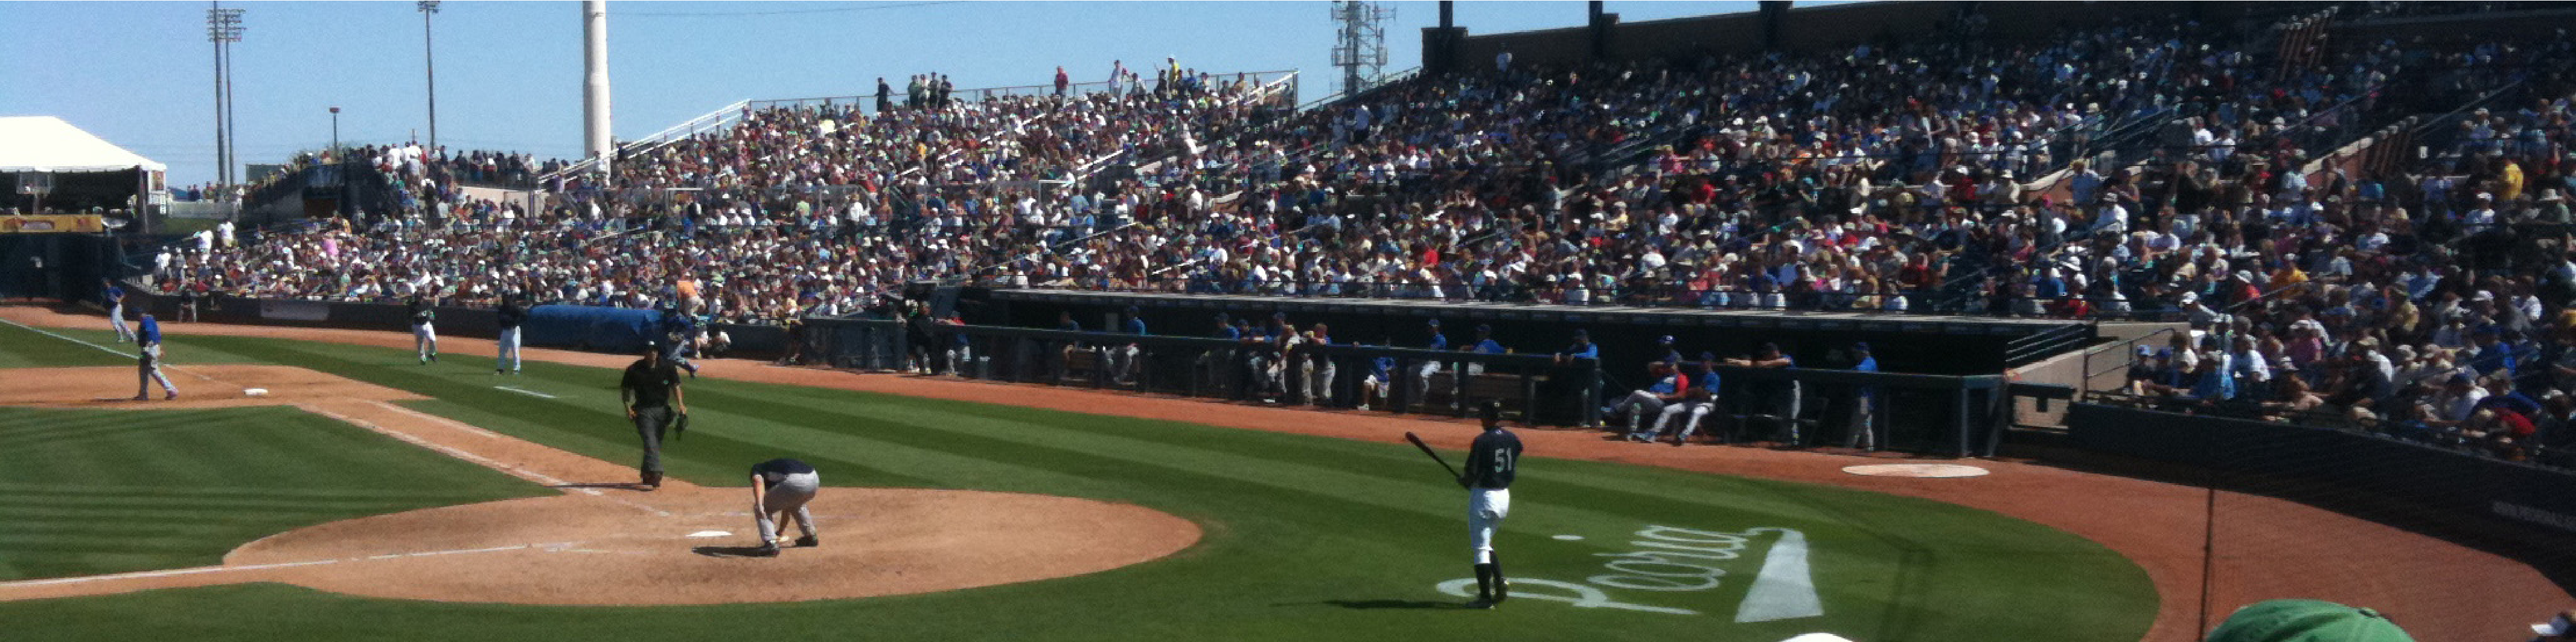
\includegraphics[width=\textwidth]{sampleteaser}
%   \caption{Seattle Mariners at Spring Training, 2010.}
%   \Description{Enjoying the baseball game from the third-base
%   seats. Ichiro Suzuki preparing to bat.}
%   \label{fig:teaser}
% \end{teaserfigure}

% \received{20 February 2007}
% \received[revised]{12 March 2009}
% \received[accepted]{5 June 2009}

%%
%% This command processes the author and affiliation and title
%% information and builds the first part of the formatted document.
\maketitle

\section{Introduction}
Fraud detection has played a crucial part in building secure products for companies that offer financial services. By clearly, efficiently, and accurately identifying fraud transactions, companies are able to prevent clients from losing money. In this project, we aim to train a model that distinguishes between legitimate and fraudulent transactions specifically on credit cards. Such models can be used by banks and online payment companies to block malicious transactions and protect their customers’ properties.

Our hypothesis is that fraudulent credit card transactions are associated with unusual patterns, and can be detected by identifying differences from a cardholder’s normal behavior and transaction characteristics.

\section{Related Work}
Financial institutions tend to use a combination of techniques and algorithms to detect fraudulent transactions, depending on the specific characteristics of the transactions. Specific client/customer data is highly private in the real world, hence we do not know the exact modeling process behind each fraud detection department of those companies. Some research papers are available, such as Credit Card Fraud Detection using Machine Learning Algorithms by V. Dornadula and S. Geetha, where they used SMOTE (an oversampling technique) and SVM (Support Vector Machine) for their model.

We aim to use this project as a practice to build a robust model with proper data cleaning and feature engineering process that will serve well when we get to work with industry-level datasets in the near future.


\section{Methods}
We performed data cleaning and feature engineering on our dataset, then compared the effect of logistic regression (baseline model), Support Vector Machine, random forest, and AdaBoost.

\subsection{Exploratory Data Analysis}
We use the dataset “Credit Card Transactions Fraud Detection Dataset” \cite{KaggleFraudDetection} found on Kaggle. The dataset is created using a simulator, but should be highly similar to a real-world dataset in credit card transactions and contains both legitimate and fraudulent credit card transactions from 1/1/2019 to 12/32/2020. It contains 1,296,675 rows of data in training set and 555,719 row of data in training set. For each row, the dataset includes 10 numeric variables and 12 categorical variables. There is only one row of missing data in the training set. Since removing it from the dataset would have minimal effect, we simply dropped the row of data with missing values. 

% \begin{figure}[h]
%   \centering
%   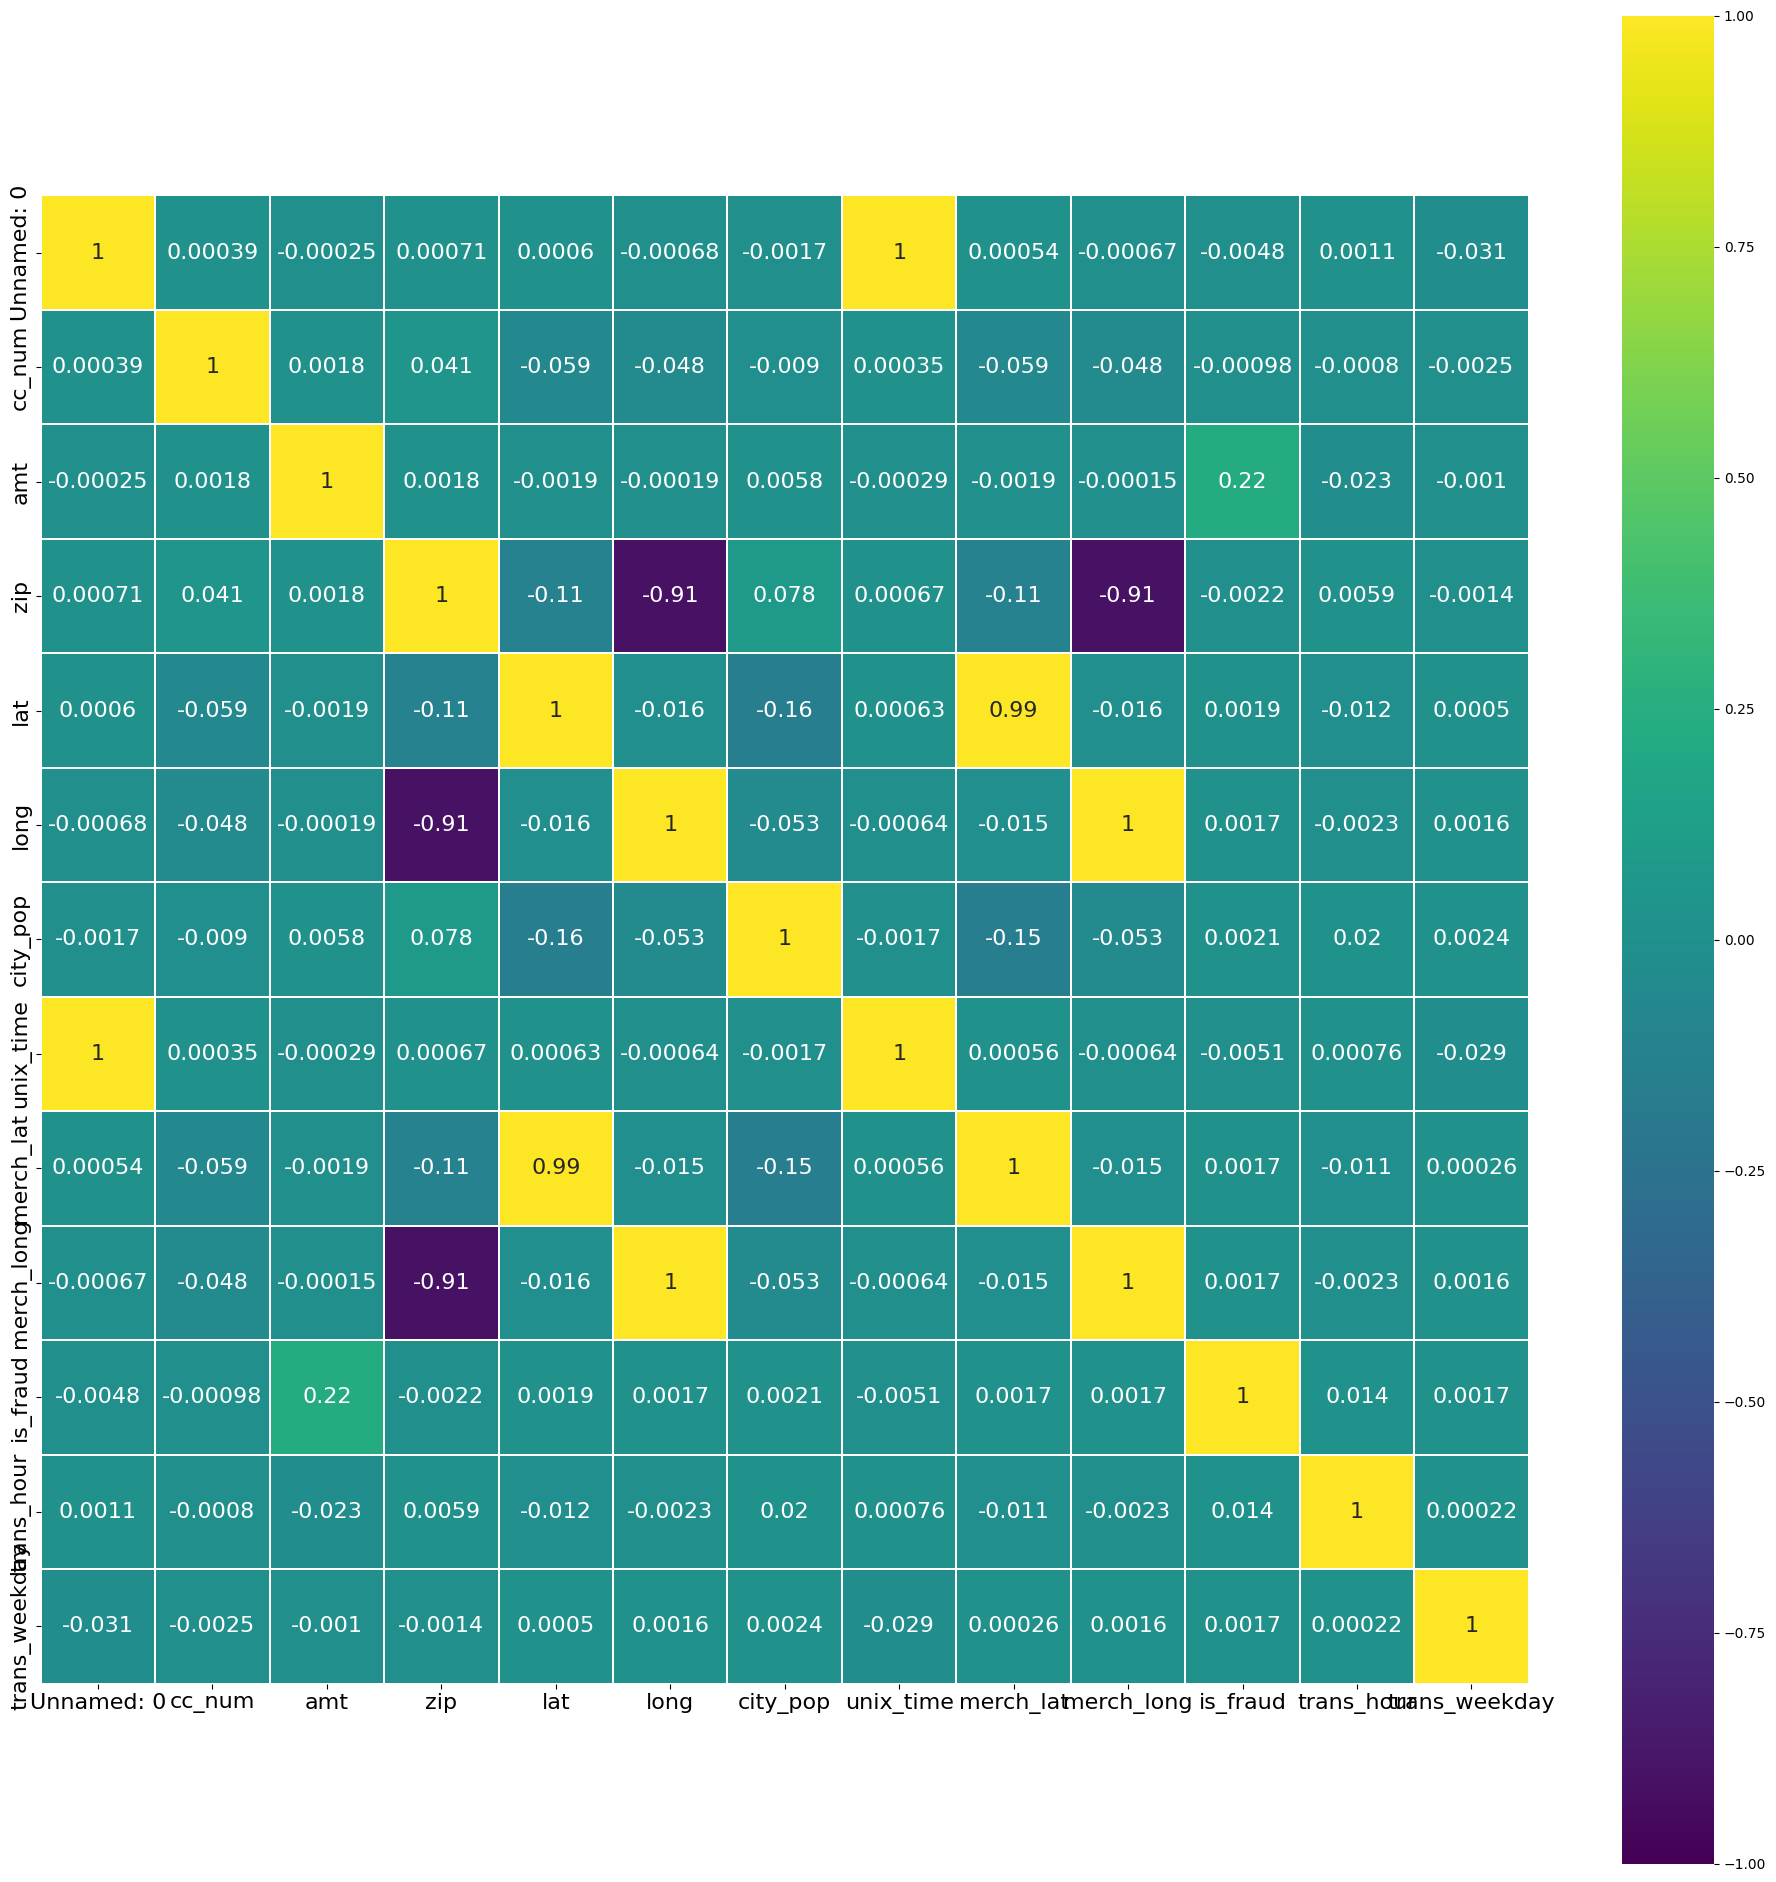
\includegraphics[width=\linewidth]{heatmap.png}
%   \caption{Heatmap between Numerical Variables and the Target Variable ``is\_fraud''}
%   % \Description{A woman and a girl in white dresses sit in an open car.}
% \end{figure}

\begin{table}
  \caption{Correlation between Numeric Variables and the Target Variable ``is\_fraud''}
  \label{tab:correlation}
  \begin{tabular}{cc}
    \toprule
        Variable Name&Correlation\\
    \midrule
        is\_fraud& 1.000000\\
        amt& 0.219404\\
        % trans\_hour& 0.013799\\
        city\_pop& 0.002136\\
        lat&0.001894\\
        merch\_lat&0.001741\\
        % trans\_weekday&0.001739\\
        merch\_long&0.001721\\
        long&0.001721\\
        cc\_num&-0.000981\\
        zip&-0.002162\\
        unix\_time&-0.005078\\
    \bottomrule
\end{tabular}
\end{table}

As shown in {\bfseries Table 1}, most numeric variables do not have a strong correlation with the target variable ``is\_fraud'' other than the variable ``transaction amount'', which has a seemingly moderate relationship with the target variable ``is\_fraud''. This indicates that standard linear models might not be able to produce the best results for this dataset. We could potentially look into tree algorithms for a better model. In addition, we also observe that some numeric variables are suitable for further feature engineering, such as variables ``cc\_num'', ``zip'', and ``unix\_time''.

We then looked at the categorical variables, but not much clear pattern is found from any individual variable. We plan to perform feature engineering on some of those variables, such as ``category'' (transaction category), ``job'' (jobs of the cardholders), ``gender''. We also found some categorical variables non-essential to our model and should be removed before we build the model. For example, categorical variables ``first'' and ``last'' record the first and last name of the cardholders and thus provide overlapping information with the customers' credit card numbers recorded in variable ``cc\_num''.

% \begin{figure}[h]
%   \centering
%   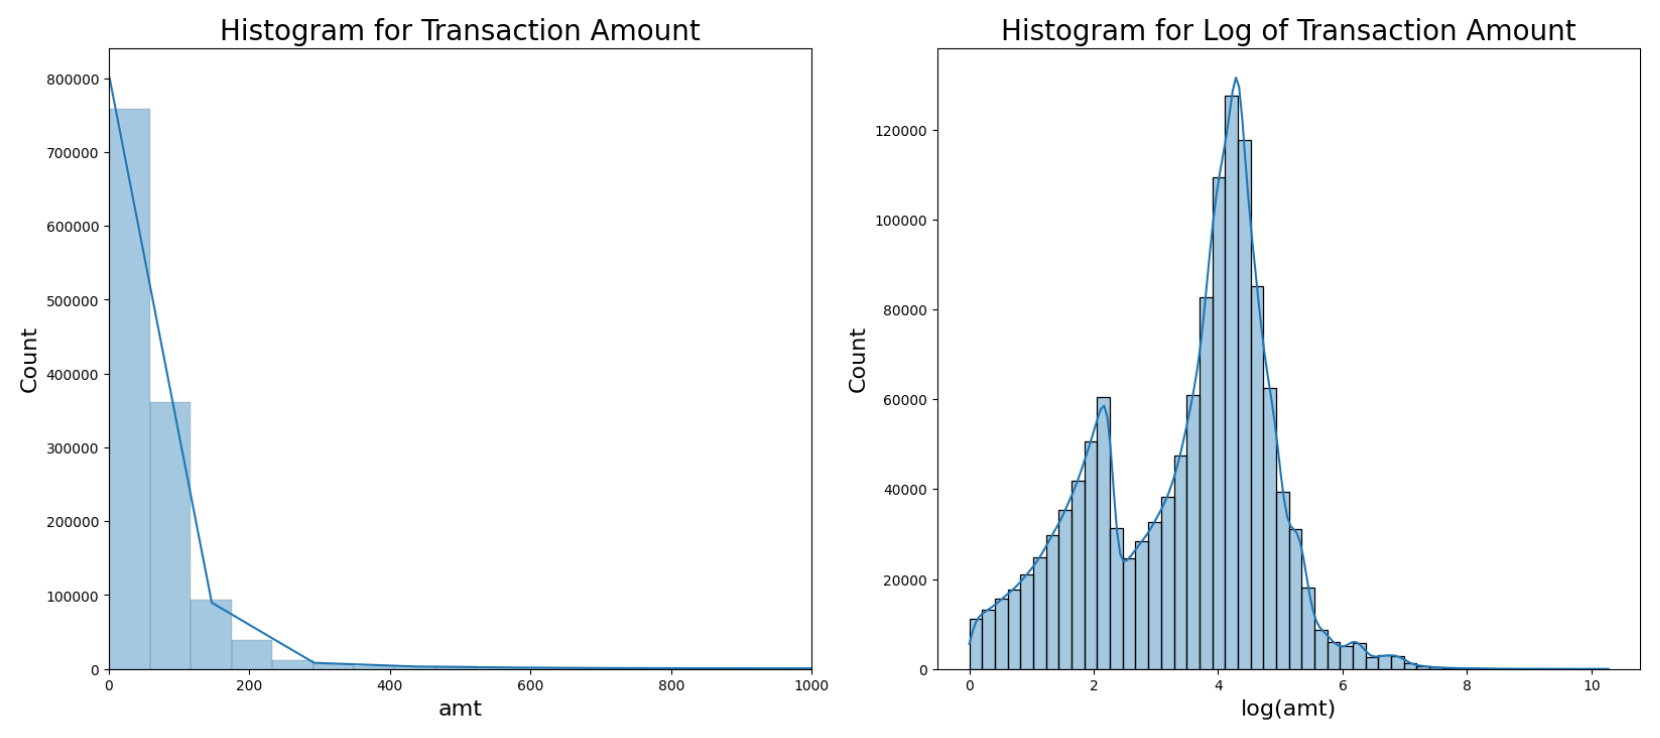
\includegraphics[width=\linewidth]{trans-amt.png}
%   \caption{Histogram for Transaction Amount, Log Transformed}
%   % \Description{A woman and a girl in white dresses sit in an open car.}
% \end{figure}


\subsection{Feature Engineering}
In our exploratory data analysis, few variables exhibited strong correlation with the target variable. Therefore, we decided to use feature engineering to create new variables based on existing dataset, tailoring them to better suit the purpose of our project. 

We first dropped columns that are unnecessary, namely ``first'', ``last'', ``street'' (street address), ``city'', ``state'', and ``trans\_num'' (identifier for each transaction). 

We then created a few new variables. The ``dob'' variable (date of birth of cardholder) was transformed into a numeric variable ``age''. We split ``unix\_time'' (time of the transaction) into ``trans\_weekday'' and ``trans\_hour'', representing the day of the week and the hour of the day of the transaction, respectively. 

After that, we applied count encoding to categorical variables ``category'', ``merchant'', ``job'', ``cc\_num'' and ``zip''. This process involved creating a new variable for each of these variables, populated with the number of occurrence of their respective categorical values. Additionally, we used one-hot-encoding on the ``gender'' variable, creating two new variables ``gender\_F'' and ``gender\_M''. 

Finally, we concluded the feature engineering phase by oversampling our target variable ``is\_fraud''. We used SMOTE (Synthetic Minority Oversampling TEchnique) to address the imbalanced distribution between fraudulent and non-fraudulent transaction data points. This prevented our models from over-fitting to the predominant non-fraudulent transaction class, thereby enhancing both the performance and robustness of our models.

\begin{figure}[h]
  \centering
  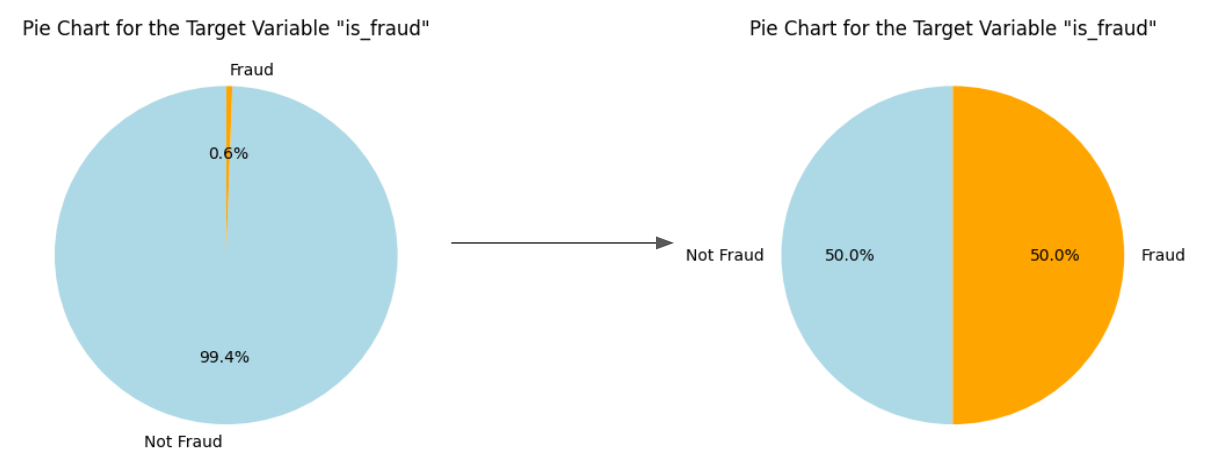
\includegraphics[width=\linewidth]{oversampling.png}
  \caption{Using SMOTE to address data imbalance}
  % \Description{A woman and a girl in white dresses sit in an open car.}
\end{figure}

\subsection{Modeling}

We used 4 different models and tried to compare their performances. 

We made logistic regression as our baseline model, since it is the most classic and fundamental algorithm for doing binary classification on datasets.

We built a support vector machine (SVM) model. SVM is a model that's been widely used in prior works related to fraud transaction detection. If SVM turns out to have good performance on the dataset, that means that there exists a clear "margin" between fraudulent and non-fraudulent transactions. 

We used 2 tree-based algorithms, random forest and Adaptive Boosting (Adaboost). Our exploratory data analysis showed that most variables do not have a strong linear correlation with the target variable, so we hope to see if we can capture nonlinear relationships between variables through training tree-based models. 

\section{Results}

We first trained the four models without tuning the hyper-parameters. The confusion matrices of the models are shown in {\bfseries Table 2}. 

\begin{table}
  \caption{Confusion Matrix Across Models, before Tuning}
  \label{tab:tn:fp:fn:tp}
  \begin{tabular}{ccccl}
    \toprule
        Model&TN&FP&FN&TP\\
    \midrule
        Logistic Regression& 5290& 254& 2&11\\
        SVM& 5411& 133& 2&11\\
        Random Forest& 5312& 232& 1&12\\
        Adaboost&5173& 371& 1&12\\
    \bottomrule
\end{tabular}
\end{table}

\begin{figure}[h]
  \centering
  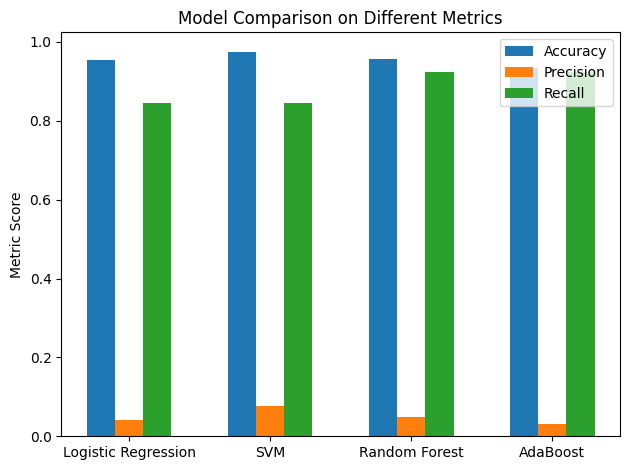
\includegraphics[width=\linewidth]{matrix comparison.png}
  \caption{Model Accuracy, Precision and Recall, before Tuning}
  % \Description{A woman and a girl in white dresses sit in an open car.}
\end{figure}

Our baseline model, the logistic regression model, achieved an accuracy of 95.4\% with a precision of 4.15\% and a recall of 84.62\%. Support Vector Machine performed the best without tuning. It achieved a 97.57\% accuracy---2.17\% higher than the baseline model, and the highest among all four models we used. The random forest model performed 0.4\% better than the baseline, with an accuracy of 95.81\%. Adaboost performed 2.1\% worse than the baseline model when we use a learning rate of 0.1 and 50 decision stumps, each with 1 decision node. We visualized the comparison between these models in {\bfseries Figure 2}.

\begin{figure}[h]
  \centering
  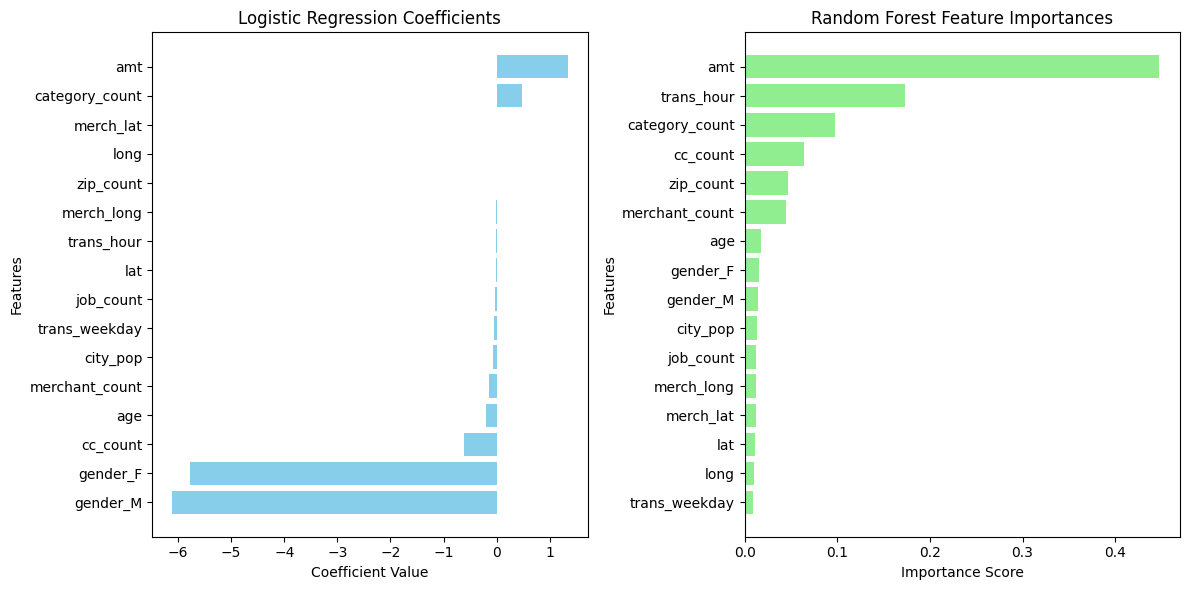
\includegraphics[width=\linewidth]{important-coeff-no-tuning.png}
  \caption{Feature Importance in Logistic Regression and Random Forest Model, before Tuning}
  % \Description{A woman and a girl in white dresses sit in an open car.}
\end{figure}

We also extracted a side-by-side histogram {\bfseries (Figure 3)} to compare the feature importance in our baseline logistic regression model and the random forest model. A few variables such as ``amt'' (transaction amount), ``category\_count'', ``zip\_count'' showed relatively high importance across both models. Additionally, the random forest was able to better utilize the count-encoded variables, such as ``category\_count'', ``cc\_count'', ``zip\_count'', and ``merchant\_count'' due to the nature of the tree-structured algorithm. 


\section{Discussion}

Before we invested our time into tuning the hyper-parameters, the SVM model and the random forest model performed better than the baseline logistic regression model. The SVM model had the highest accuracy on the testing dataset among all four models we used. However, training the model took more time than the others, and the result can be hard to interpret and visualize the model in higher dimensions, unless we use Principal Component Analysis (PCA). Meanwhile, the random forest model performs well in that it built a great balance between accuracy (95.81\%), precision (4.92\%), and recall (92.31\%).  Besides, as shown in {\bfseries Figure 3}, it was able to capture information contained by the variables created via count-encoding. However, we believe we can further improve this model via hyper-parameter tuning.

\section{Conclusion}

\section{Contribution}

% \section{References}

\bibliographystyle{ACM-Reference-Format}
\bibliography{reference}



% \section{Introduction}
% ACM's consolidated article template, introduced in 2017, provides a
% consistent \LaTeX\ style for use across ACM publications, and
% incorporates accessibility and metadata-extraction functionality
% necessary for future Digital Library endeavors. Numerous ACM and
% SIG-specific \LaTeX\ templates have been examined, and their unique
% features incorporated into this single new template.

% If you are new to publishing with ACM, this document is a valuable
% guide to the process of preparing your work for publication. If you
% have published with ACM before, this document provides insight and
% instruction into more recent changes to the article template.

% The ``\verb|acmart|'' document class can be used to prepare articles
% for any ACM publication --- conference or journal, and for any stage
% of publication, from review to final ``camera-ready'' copy, to the
% author's own version, with {\itshape very} few changes to the source.

% \section{CCS Concepts and User-Defined Keywords}

% Two elements of the ``acmart'' document class provide powerful
% taxonomic tools for you to help readers find your work in an online
% search.

% The ACM Computing Classification System ---
% \url{https://www.acm.org/publications/class-2012} --- is a set of
% classifiers and concepts that describe the computing
% discipline. Authors can select entries from this classification
% system, via \url{https://dl.acm.org/ccs/ccs.cfm}, and generate the
% commands to be included in the \LaTeX\ source.

% User-defined keywords are a comma-separated list of words and phrases
% of the authors' choosing, providing a more flexible way of describing
% the research being presented.

% CCS concepts and user-defined keywords are required for for all
% articles over two pages in length, and are optional for one- and
% two-page articles (or abstracts).


% \section{Math Equations}
% You may want to display math equations in three distinct styles:
% inline, numbered or non-numbered display.  Each of the three are
% discussed in the next sections.

% \subsection{Inline (In-text) Equations}
% A formula that appears in the running text is called an inline or
% in-text formula.  It is produced by the \textbf{math} environment,
% which can be invoked with the usual
% \texttt{{\char'134}begin\,\ldots{\char'134}end} construction or with
% the short form \texttt{\$\,\ldots\$}. You can use any of the symbols
% and structures, from $\alpha$ to $\omega$, available in
% \LaTeX~\cite{Lamport:LaTeX}; this section will simply show a few
% examples of in-text equations in context. Notice how this equation:
% \begin{math}
%   \lim_{n\rightarrow \infty}x=0
% \end{math},
% set here in in-line math style, looks slightly different when
% set in display style.  (See next section).

% \subsection{Display Equations}
% A numbered display equation---one set off by vertical space from the
% text and centered horizontally---is produced by the \textbf{equation}
% environment. An unnumbered display equation is produced by the
% \textbf{displaymath} environment.

% Again, in either environment, you can use any of the symbols and
% structures available in \LaTeX\@; this section will just give a couple
% of examples of display equations in context.  First, consider the
% equation, shown as an inline equation above:
% \begin{equation}
%   \lim_{n\rightarrow \infty}x=0
% \end{equation}
% Notice how it is formatted somewhat differently in
% the \textbf{displaymath}
% environment.  Now, we'll enter an unnumbered equation:
% \begin{displaymath}
%   \sum_{i=0}^{\infty} x + 1
% \end{displaymath}
% and follow it with another numbered equation:
% \begin{equation}
%   \sum_{i=0}^{\infty}x_i=\int_{0}^{\pi+2} f
% \end{equation}
% just to demonstrate \LaTeX's able handling of numbering.

% \section{Appendices}

% If your work needs an appendix, add it before the
% ``\verb|\end{document}|'' command at the conclusion of your source
% document.

% Start the appendix with the ``\verb|appendix|'' command:
% \begin{verbatim}
%   \appendix
% \end{verbatim}
% and note that in the appendix, sections are lettered, not
% numbered. This document has two appendices, demonstrating the section
% and subsection identification method.

% \section{SIGCHI Extended Abstracts}

% The ``\verb|sigchi-a|'' template style (available only in \LaTeX\ and
% not in Word) produces a landscape-orientation formatted article, with
% a wide left margin. Three environments are available for use with the
% ``\verb|sigchi-a|'' template style, and produce formatted output in
% the margin:
% \begin{itemize}
% \item {\verb|sidebar|}:  Place formatted text in the margin.
% \item {\verb|marginfigure|}: Place a figure in the margin.
% \item {\verb|margintable|}: Place a table in the margin.
% \end{itemize}

% %%
% %% The acknowledgments section is defined using the "acks" environment
% %% (and NOT an unnumbered section). This ensures the proper
% %% identification of the section in the article metadata, and the
% %% consistent spelling of the heading.
% \begin{acks}
% To Robert, for the bagels and explaining CMYK and color spaces.
% \end{acks}

% %%
% %% The next two lines define the bibliography style to be used, and
% %% the bibliography file.
% % \bibliographystyle{ACM-Reference-Format}
% % \bibliography{reference}

% %%
% %% If your work has an appendix, this is the place to put it.
% \appendix

% \section{Research Methods}

% \subsection{Part One}

% Lorem ipsum dolor sit amet, consectetur adipiscing elit. Morbi
% malesuada, quam in pulvinar varius, metus nunc fermentum urna, id
% sollicitudin purus odio sit amet enim. Aliquam ullamcorper eu ipsum
% vel mollis. Curabitur quis dictum nisl. Phasellus vel semper risus, et
% lacinia dolor. Integer ultricies commodo sem nec semper.

% \subsection{Part Two}

% Etiam commodo feugiat nisl pulvinar pellentesque. Etiam auctor sodales
% ligula, non varius nibh pulvinar semper. Suspendisse nec lectus non
% ipsum convallis congue hendrerit vitae sapien. Donec at laoreet
% eros. Vivamus non purus placerat, scelerisque diam eu, cursus
% ante. Etiam aliquam tortor auctor efficitur mattis.

% \section{Online Resources}

% Nam id fermentum dui. Suspendisse sagittis tortor a nulla mollis, in
% pulvinar ex pretium. Sed interdum orci quis metus euismod, et sagittis
% enim maximus. Vestibulum gravida massa ut felis suscipit
% congue. Quisque mattis elit a risus ultrices commodo venenatis eget
% dui. Etiam sagittis eleifend elementum.

% Nam interdum magna at lectus dignissim, ac dignissim lorem
% rhoncus. Maecenas eu arcu ac neque placerat aliquam. Nunc pulvinar
% massa et mattis lacinia.

\end{document}
\endinput
%%
%% End of file `sample-authordraft.tex'.
